\section{Irrigation in the world and in the Iberian Peninsula}
Irrigation is a widespread practice in the world which consists in providing additional water to cultivated soil to favor crop growth and development.
Irrigated fields are estimated to cover about 20\% of global cropland (3.5 million km$^2$), which account for 40\% of the food produced in the world.

This practice is widespread globally in various forms (gravity irrigation, sprinklers, drip irrigation) and enables agriculture to maintain yields that would not be achievable in many regions otherwise. The historical reconstruction by \citet{siebert_global_2015} estimates that the total irrigated area increased fivefold during the 20th century due to population growth and industrialization, rising from 63 Mha in 1900 to 306 Mha in 2005. Certain regions stand out, such as South Asia, the Western United States, Eastern China, and Western Europe (Figure \ref{irrig_evolution_map}).

\begin{figure}[ht]
    \centering
    
\includegraphics[width=\textwidth]{images/intro/irrig_evolution_Siebert.png}
    \caption{Percentage of area equipped for irrigation in 1900, 1960, and 2005 according to the HID (Historical Irrigation Dataset). Extracted from \citet{siebert_global_2015}.}
    \label{irrig_evolution_map}
\end{figure}

%various methods : flooding, sprinkler, drip
%various sources : river, dams, pumping, advection from mountainous areas
%order of magnitudes : world fraction, volumes / same for Spain+Portugal
%how it's estimated ?

\section{Climate modelling}
Climatology aims at describing statistical distribution of multiple variables of interest, among which temperature, pressure, humidity, precipitation, and wind speed.
For centuries, it remained a science based on observations, 
%todo : koppen geiger

which then led to the formulation of conceptual models and to mathematical representations of the energy balance and radiative tranfer processes.
%todo cite Edwards
The Navier-Stokes equations describe the fluid mechanics that control the motions of the atmosphere. However these equations do not have any known analytical solution, forbidding their direct use to predict motions of air, water and other components of the atmosphere. 
Modern climate modelling originated in the 1950s with the development of computer simulations which enable numerically estimating solutions of these equations.

%todo: cite Manabe, others ?
General circulation models (GCMs) use a simplified version of the Navier-Stokes equations, referred to as \textit{primitive equations}, to represent the complex motions of the atmosphere. 
The globe is discretized into grid cells, which can range from a few tens to a few hundred kilometers. Using an appropriate temporal discretization, this enables approximating solutions of the primitive equations to represent atmospheric dynamics. This part of the model is often referred to as \textit{the dynamical core}. However, several major processes of the climate system are not described by fluid mechanics and require additional \textit{parameterizations}, which compute the mean effect of various processes in each vertical column, independently of neighbouring grid cells. Most importantly, they represent all radiative emission and transfer processes which largely dictate the energy budget of the atmosphere.
Thermodynamic processes involved in the phase changes of water are also essential to represent energy transfers between phases, cloud formation and precipitation. Parameterizations are also used to account for the processes that occur at a smaller scale than the resolution of the GCM and cannot be described by the dynamical core, such as turbulent diffusion or shallow and deep convection processes. Finally, parametererization are used to represent interactions of the atmosphere with the various surfaces it can be interfaced with: sea surface, ice caps or sea ice, bare soil, vegetation, urban areas... Interactions between the land surface and the atmosphere and the feedback loops between the two systems are a major focus of this thesis, and the following section %tocheck
provides a detailed description of the state of knowledge in this field. 


\begin{figure}[ht]
    \centering
    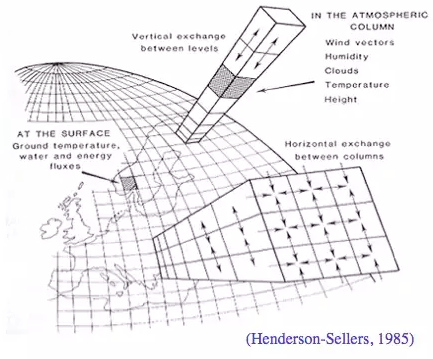
\includegraphics[width=\textwidth]{images/intro/GCM_structure.png}
    \caption{GCM structure %todo:ref
    }
    \label{fig:GCM}
\end{figure}


Historically, the first climate models primarily focused on the atmosphere, with
a very simplified representation of the surface. Over the past three decades, climate models have evolved to distincly represent continental surfaces by coupling atmospheric models with ocean models and land surface models (LSMs), and are now often referred to as Earth system models (ESMs). Nowadays, ESMs are not only used to simulate temperature, precipitation, and wind, but can have a much wider range of applications in geoscience, paleoclimatology, oceanography, glaciology, subsurface hydrology, biology, biogeochemistry, etc... 
Regarding land surface in particular, the complexity of LSMs has gradually increased, for example, to better account for the influence of vegetation on the atmosphere, or to represent additional processes of interest such as rivers and groundwater, and biogeochemical cycles of carbon or nitrogen. They can also be used as standalone models using atmospheric forcings instead of a dynamical coupling with a GCM.

%limits to increase in resolution : computing power, physical hypotheses
%how do we evaluate them : point based and satelite obs

%specificities of regional modelling ? Lateral forcing
%mention hierarchy of models, CRM/mesoscale/NWP, RANS/LES, (DNS)

% notion of climate variability, sensitivity to initial (+/- boundary conditions). Idea that running a climate model over a given year may not represent correctly what happenned on that year, but that over a decade (or more) it should be able to reproduce the mean state of climate.

\subsection{Climate change}
As early as 1824, Joseph Fourier, followed by Claude Pouillet, theoretized than some atmospheric components of the atmosphere can influence the temperature of the air more than others, which was demonstrated in 1838 by Eunice Newton Foote for water vapour and carbon dioxyde (CO2). This was linked to infrared absorption and emissions by the experimental work of John Tyndall, and, in 1896, Svante Arrhenius conducted the first estimate of the global temperature increase caused by a hypothetical doubling of CO2 in the atmosphere.

Since the industrial revolution in the 19th century, anthropic activities have increased %todo : estimate
the amounts of greenhouse gases in the atmosphere, mainly as a consequence of fossil fuel combustion and by destruction of natural sinks to give way to agricultural land.
By the end of the 1950s, it was established that concentration of CO2 in the atmosphere was increasing, %todo: cite and show Keeling curve
and that although water vapour was overwhelmingly dominant in the atmospheric composition, other greenhouse gases present in the upper atmosphere, such as CO2, could have a significant impact on global energy balance, and therefore temperature. Therefore, concerns arose about the possible rise of global temperatures and the impacts it could have on natural ecosystems and human activities.
Concurrent research in paleoclimatology showed that previous evolutions of greenhouse gases in the atmosphere had never been this fast, and were all associated with large-scale changes. 

As this knowledge progressed coincidentally with modelling capablilities in numerical climate modelling, models started to be used not only to reproduce past and present climate, but also to simulate future climate scenarios. They quickly confirmed the risk of rapid increases in global temperature, and hinted at the global and regional consequences on ice cap and glacier melting, sea level rise, and disruption of the water cycle among others. In 1988, the International Panel on Climate Change was established by the World Meteorological Organisation (WMO) and the United Nations Environment Program (UNEP) to unify efforts in climate change science, and on the socio-economic impacts of global warming. This group still carries on today in its mission to "provide governments at all levels with scientific information that they can use to develop climate policies".

At the end of the 20th and the beginning of the 21st centuries, there were also many developments in the field of remote sensing which enabled the monitoring of climate variables from satellites. 


%SSP emission pathways

\section{Land-atmosphere interactions}

Over land, interactions between the surface and the lower layers of the atmosphere have significant impacts on meteorological (air temperature and humidity, precipitation, wind) and hydrological (runoff, stream flow, soil moisture) variables. The two systems influence each other's water and energy budgets, and multiple feedback loops can be identified depending on the spatial and temporal scales considered. The complexity of this coupling and the variety of impacts it can have on ecosystems and human activities make it a subject of interest for climate science and a necessary component of climate or numerical weather prediction (NWP) models. This section aims to provide a state-of-the-art description of these interactions and their modelling, as well as the impacts irrigation can have on them.

\subsection{Water and energy budgets at the surface}
To understand the components of the land-atmosphere coupling, it is necessary to recall the main fluxes of water and energy at the surface. 
Figure \ref{fig:budgets} depicts the various components of these two budgets.

\begin{figure}[ht]
    \centering
    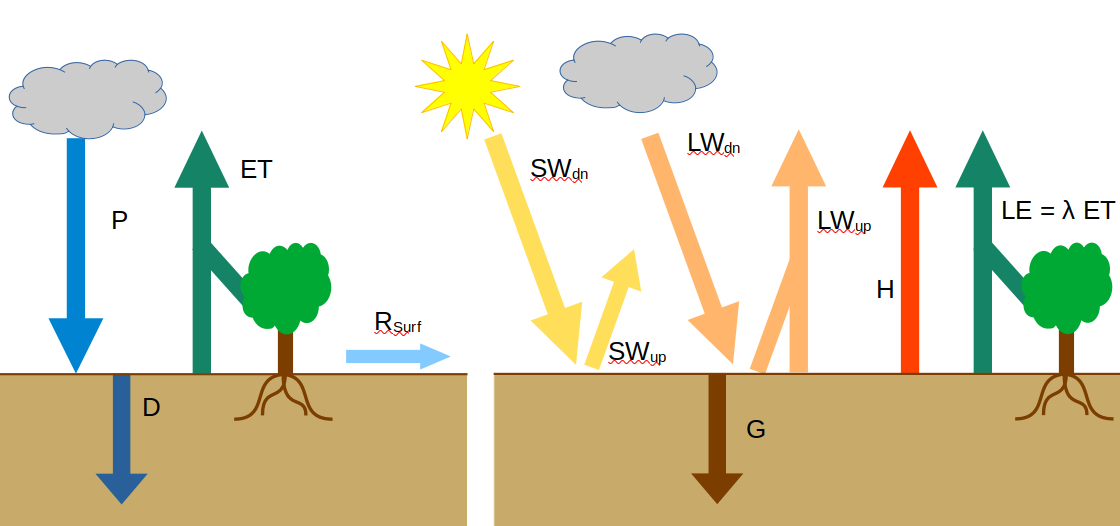
\includegraphics[width=\textwidth]{images/intro/budgets.png}
    \caption{Surface water and energy budgets. \\Based on similar figures from \citet{seneviratne_investigating_2010}%add these tanguy
    }
    \label{fig:budgets}
\end{figure}

The surface water budget accounts for:
\begin{itemize}
    \item Precipitation (transfer from the atmosphere to the surface), $P$.
    \item Evapotranspiration (transfer of liquid or solid water from the surface to the atmosphere in gaseous form), $ET$. It is the sum of direct evaporation and of transpiration, a process in  which vegetation releases water is has collected in the soil.
    \item Drainage of water in the soil to lower layers, denoted  as $D$. 
    \item Surface runoff, $R_{surf}$, water that does not infiltrate in the soil and flows out of the area considered.
\end{itemize}

The equation governing the evolution of water quantity in the upper soil layer (denoted here as $W$) is:
\begin{equation}
    \frac{dW}{dt} = P - ET - R_{surf} - D
\end{equation}

The surface energy budget includes:
\begin{itemize}
    \item Shortwave radiation (SW), with an incoming term ($SW_{dn}$) corresponding to incident solar radiation and an outgoing term ($SW_{up}$) corresponding to the portion reflected by the surface .

    The difference between these two terms and the albedo of the considered surface are defined as:

    $SW_{net} = SW_{dn} - SW_{up}$

    $\alpha_{SW} = SW_{up}/SW_{dn}$.
    \item Longwave radiation (LW), with an incoming term ($LW_{dn}$) corresponding to the infrared radiation reflected or emitted by clouds and atmospheric gases reaching the surface and an outgoing term ($LW_{up}$) corresponding mostly to the infrared radiation emitted by the surface based on its temperature, as well as a partial reflection of the incoming LW radiation.

    The difference between these two terms is defined as $LW_{net} = LW_{dn} - LW_{up}$.
    
    The net radiation is also defined as the sum of the two radiation terms: $R_{n} = SW_{net} + LW_{net}$.
    \item Sensible heat flux $H$, which is a thermal transfer between the air and the surface.
    \item Latent heat flux, which corresponds to the energy used to evaporate water at the surface. This energy flux is directly related to evapotranspiration (water flux) through the enthalpy of vaporization ($\lambda$), and is therefore denoted as $LE = \lambda ET$.
    \item Heat flux to the soil, which is a thermal conduction transfer between the considered surface layer and the lower soil layers, denoted as $G$.
\end{itemize}

The equation governing the evolution of energy in the surface soil layer (denoted as $E$ in Figure \ref{fig:budgets}) is:
\begin{equation}
    \frac{dE}{dt} = R_{n} - G - \lambda ET - H
\end{equation}

\subsection{Role of soil moisture in land-atmosphere interactions}

The term \textit{coupling} between the surface and the atmosphere encompasses multiple influences and feedbacks between the two systems. Soil moisture plays a central role in this coupling through its direct and indirect interactions with evapotranspiration, precipitation, and the surface energy budget.

\subsubsection*{Atmospheric boundary layer development and air temperature}

In meteorology, the atmospheric boundary layer (ABL) is defined as the lower part of the troposphere directly influenced by the presence of the surface. This layer is where shallow convection and turbulent diffusion phenomena occur, contributing to energy diffusion and mixing of the air.
The lowest part of the boundary layer, on the order of a few tens of meters, is called the surface layer. The influence of the Coriolis force is negligible compared to that of the surface, and the wind speed generally follows a logarithmic profile. The empirical similarity theory developed by Monin and Obukhov describes the mean flow, temperature, and humidity in this layer \citep{monin1954osnovnye}.
The height of the boundary layer varies during the diurnal cycle depending on air stability, which is related to the presence of vertical temperature and humidity gradients, and wind. It can measure a few tens of meters at night and up to a few kilometers during the day in arid regions \citep{garratt_review_1994}.

The partitionning of energy between the two turbulent fluxes at the surface ($\lambda ET$ and $H$) plays an essential role in the development of the boundary layer. As a tought experiment, for a given net radiation $R_n$ and a nearly constant soil heat flux (e.g., over 24 hours if there is equilibrium between daytime and nighttime), the remaining energy is distributed between the two turbulent fluxes. The evaporative fraction (defined as $EF = \lambda ET / R_n$) %attention défini autrement dans l'article EF=LE/(LE+H)
and the Bowen ratio (defined as $B = H / \lambda ET$) quantify this partitionning. If the latent heat flux is very high compared to the sensible heat flux ($EF$ high, $B$ low), the air temperature in the surface layer remains low because the energy is primarily used for evapotranspiration, and the soil transfers little heat to the air. Conversely, if the Bowen ratio is high, a larger portion of the incident energy is transmitted directly to the air, leading to a higher air temperature near the surface and more pronounced development of the boundary layer \citep{betts_fife_1995}.
In reality, the processes are a bit more complex since the surface temperature (and therefore the $LW_{up}$ flux) may also react to changes in latent heat flux, but the reciprocal behaviour of the latent and sensible heat fluxes has been identified in multiple observations and modelling experiments \citep{betts_fife_1995, seneviratne_investigating_2010}. %todo:source

Moreover, soil moisture also affects the thermal properties of the soil, as wet soil has greater thermal inertia than dry soil. In contexts where the latent heat flux is limited, this can significantly impact air temperature by affecting nighttime cooling \citep{ait-mesbah_role_2015}. The absence of solar radiation at night usually leads to radiative cooling of the soil and air in the surface layer. However, for wetter soil, this cooling will be less pronounced due to higher thermal inertia. During daytime, the impact of this inertia is often negligible, and other processes dominate the evolution of air temperature. Still, on a daily average, an increase in soil moisture can lead to an increase in air temperature since nighttime cooling is less significant \citep{cheruy_role_2017}.

\subsubsection*{Coupling between soil moisture and evapotranspiration}

Soil moisture is a key factor in the description of evapotranspiration regimes initially established by \citet{Budyko_1956, Budyko_1974}. Three main regimes are identified for the evolution of the evaporative fraction $EF$. Figure \ref{fig:evap_regimes} represents these regimes.

\begin{itemize}
    \item If soil moisture is below a threshold $\theta_{WILT}$, called the wilting point, plants cannot extract water to transpire, bare soil no longer evaporates, and evapotranspiration (and thus the evaporative fraction) is zero. This first regime is called the \textbf{dry regime}.
    \item If soil moisture is above a critical threshold $\theta_{CRIT}$, soil moisture has no impact on $EF$, which is maximal. Evaporation is limited by the available incident energy, it is the \textbf{wet regime}.
    \item Between $\theta_{WILT}$ and $\theta_{CRIT}$, there is a \textbf{transition regime} where evapotranspiration is primarily conditioned by soil moisture. As in the dry regime, evapotranspiration is limited by soil moisture.
\end{itemize}

\begin{figure}[ht]
    \centering
    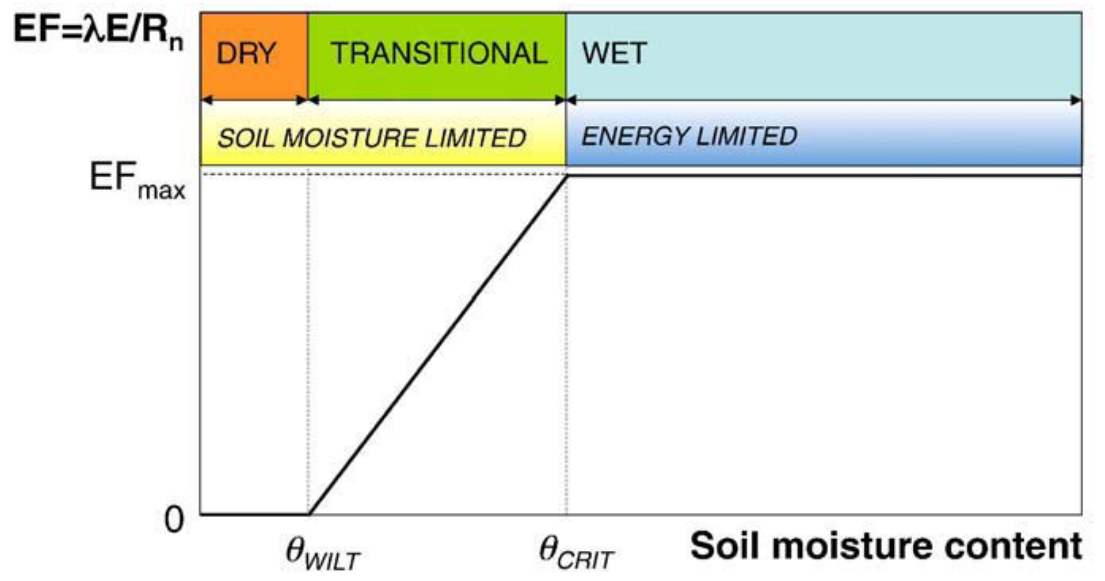
\includegraphics[width=0.7\textwidth]{images/intro/evap_regimes.png}
    \caption{Representation of different evapotranspiration regimes. Extracted from \citet{seneviratne_investigating_2010}.}
    \label{fig:evap_regimes}
\end{figure}

Through its influence on evapotranspiration, soil moisture directly impacts surface water and energy budgets, particularly the distribution of energy between turbulent fluxes. As explained earlier, this has consequences for air temperature and humidity in the surface layer.

However, there are also several the feedbacks of evapotranspiration on soil moisture. First, an increase in evapotranspiration directly leads to a decrease in soil moisture and an increase in air humidity. This contributes to reducing the vertical humidity gradient between the air and the surface, which tends to limit evaporation \citep{allen_crop_2000}, forming a negative feedback loop. It is also established that an increase in air temperature leads to higher evaporative demand \citep{jarvis_stomatal_1986}. If enough water is available in the soil, a temperature increase will increase evapotranspiration, thus decreasing soil moisture. This can form a positive feedback loop where dry soil leads to high air temperatures, resulting in even drier soil and possibly initiating extreme drought events \citep{quesada_asymmetric_2012}. If no more water is available or if there are no more gradients between the soil surface and the air, the feedback of air temperature on soil moisture becomes neutral, and the feedback loop is interrupted.

\subsubsection*{Coupling between soil moisture and precipitation}

The most complex processes of surface-atmosphere coupling concern the link between soil moisture and precipitation. Several opposing effects are at play, with a large importance of spatial heterogeneities of soil moisture at the surface, which may derive from the diversity of vegetation, soil types, orographic features, and anthropogenic processes.

Increases in SM and ET have been associated with direct increases in precipitation in both modelling and observational studies \citep{koster_observational_2003, guo_glace_2006, wei_dissecting_2012, findell_probability_2011}, constituting a positive feedback loop \citep[moisture recycling, as presented in ][]{eltahir_precipitation_1996}.

However, high soil moisture can lead to a stabilisation of the boundary layer. %todo:citation ? details ? mention that it's driven by H ?
This stabilisation can inhibit vertical development and convective processes involved in cloud formationa and precipitation \citep{findell_atmospheric_2003-1, ek_influence_2004}. 
This constitutes a negative feedback loop where convective rainfall is more likely to occur over drier soil patches, which was noticed in observations \citep{taylor_afternoon_2012, klein_dry_2020}. These findings suggest that indirect processes related to boundary layer structure and heterogeneities can locally exceed the direct process of atmospheric moisture recycling, although demonstrating causality in such observational studies remains challenging \citep{salvucci_investigating_2002, guillod_land-surface_2014}. Building on the purely spatial analysis of \citet{taylor_afternoon_2012}, a spatiotemporal analysis of correlations between soil moisture and precipitation highlighted the importance of temporal variability \citep{guillod_reconciling_2015}. It showed that while precipitation is more frequently triggered over drier areas, it occurs on days that are wetter relative to the season and region concerned.
Finally, spatial heterogeneities in soil moisture have also been identified as factors influencing precipitation through mesoscale circulations that can either favour or inhibit convection triggering \citep{findell_atmospheric_2003, taylor_frequency_2011, rochetin_morphology_2017}.

\subsection{Land-atmosphere interactions in climate models}

In modern ESMs of NWP models %todo:check que NWP défini avant
he modelling of land-atmosphere interactions involves both the atmospheric model and the land surface model, and the modelling choices for their coupling.
From the perspective of an atmospheric model, latent and sensible heat fluxes at the surface constitute necessary boundary conditions for solving turbulent diffusion equations throughout the considered atmospheric column. These conditions impact essential meteorological variables such as air temperature, wind, and humidity. From the perspective of the LSM, precipitation computed in the atmospheric model constitutes a water input for the soil column, while surface layer characteristics (humidity, temperature, wind) condition evapotranspiration demand.

Various experiments have been designed to quantify the importance of surface coupling processes for atmospheric models. In particular, the GLACE experiments \citep{koster_glace_2006} compared atmospheric simulations with different prescribed soil moisture conditions to isolate the influence of soil moisture on precipitation. This led to the identification of hotspots: regions where this coupling is particularly pronounced. These are mainly semi-arid regions (Sahel, Great Plains in the United States) where the transitional evaporation regime described in Figure \ref{fig:evap_regimes} is more frequent than dry and wet regimes \citep{koster_regions_2004}.
This was confirmed by other modelling studies that also identified various mechanisms through which land surface conditions can impact the atmosphere in these coupling hotspots, and metrics to quantify them \citep{dirmeyer_terrestrial_2011, zou_precipitation_2023}.
The GLACE-CMIP5 experiments \citep{seneviratne_impact_2013} extended these conclusions by highlighting the importance of this coupling in the global warming response observed in these hotspots \citep{berg_interannual_2015}.

A particular challenge in modelling this coupling within an ESM arises from the size of the grid cells used (generally around 100 km for long climate simulations). At this scale, numerous subgrid heterogeneities exist at the surface, requiring the aggregation and averaging of highly diverse land-atmosphere interactions depending on vegetation cover, elevation, or anthropogenic factors (cities, irrigation).

For example, regarding the triggering of convective rainfall in heterogeneous areas, \citet{moon_soil_2019} showed that CMIP5 models correctly reproduced the positive temporal feedbacks (rain on wetter days) described in \citet{guillod_reconciling_2015} but not the negative spatial feedbacks identified in \citet{taylor_afternoon_2012}. The influence of resolution and parametrization choices (especially for deep convection) on the importance of land-atmosphere coupling in models has also been highlighted by \citet{tuinenburg_high-resolution_2020} and \citet{lee_weaker_2024}.

Several ongoing projects aim to better document the impact of these heterogeneities and explore ways to better account for them in models. This is the case of the Land Surface Interactions with the Atmosphere over the Iberian Semi-Arid Environment (LIAISE, \cite{boone_land_2019}) and Models and Observations for Surface-Atmosphere Interactions (MOSAI, \cite{lohou_model_2022}) projects, which rely on measurement campaigns specifically dedicated to studying land-atmosphere interactions and comparing multiple models with these observations.

It is now well known that accurately representing surface-atmosphere couplings is essential for accurately representing climate, particularly temperature and precipitation extremes \citep{jaeger_impact_2011, van_den_hurk_acceleration_2011}. Furthermore, the study of CMIP5 simulations has revealed a warm bias in most models, particularly in the Mediterranean basin \citep{christensen_temperature_2012, mueller_systematic_2014}. By comparing CMIP5 model biases with satellite observations, \citet{al-yaari_satellite-based_2019} also showed that these temperature biases are correlated with soil moisture biases. More generally, surface interaction processes have been identified as a crucial factor in the appearance of these biases, especially the partitioning of energy between latent and sensible heat fluxes and the underestimation of evapotranspiration \citep{cheruy_combined_2013, cheruy_role_2014}. 

\subsection{Impacts of irrigation on land-atmosphere interactions}

Human activities can influence the various components of land-atmosphere coupling. This is particularly the case with irrigation, which directly modifies soil moisture through artificial water inputs and can create strong spatial heterogeneities in SM. 

Observational studies have established that irrigation leads to a moister and cooler atmosphere near the surface \citep{bonfils_empirical_2007, mcdermid_irrigation_2023}, which is explained by an increase in the latent heat flux and a decrease in the sensible heat flux in irrigated areas \citep{rappin_landatmosphere_2022, boone_land_2025}.
Based on observation records in California, \citet{bonfils_empirical_2007} estimated a decrease of 1.8 to 3°C in the average summer temperature since the development of irrigation practices. This cooling effect can limit temperature values during extreme meteorological events \citep{thiery_present-day_2017, thiery_warming_2020}. However, the cooling due to increased latent heat flux can be partially compensated on a daily scale by a weakening of nighttime cooling due to thermal inertia \citep{chen_irrigation_2018}.
In the American Midwest, \cite{nocco_observation_2019} showed that such effects could impact the regional climate and even mask the rise in temperature induced by global warming. Different regional responses of precipitation have also been observed, such as a decrease in irrigated areas \citep{alter_rainfall_2015} or an increase in downwind regions \citep{deangelis_evidence_2010}.
The other impacts on the atmosphere (structure of the boundary layer, mesoscale circulations, precipitation) are more complex to characterize because they do not always occur solely over the irrigated area.

To get more insights than what point-based obersvation provide and analyse the atmospheric processes involved, mesoscale modelling studies have often been used to complement observational campaigns. 
The Great Plains irrigation experiment \cite[GRAINEX,][]{rappin_great_2021} measurements and simulations with the Weather Research and Forecasting (WRF) model revealed a lower ABL over irrigated areas and a reduction of existing mesoscale slope-induced circulations in the presence of irrigation \citep{rappin_landatmosphere_2022, phillips_influence_2022}. 
In the Ebro Valley (northern Spain), Meso-NH simulations at 2-km and 400-m resolution were conducted over the area of the Land surface Interactions with the Atmosphere over the Iberian semi-arid Environment campaign \citep[LIAISE][]{boone_land_2019}. They reproduced the observed differences between irrigated areas and neighboring areas in turbulent fluxes and air temperature and were greatly improved by representing irrigation \citep{lunel_irrigation_2024}. They also highlighted a weakening of the regional sea-breeze regime due to irrigation, which reduces the pressure gradient force \citep{lunel_marinada_2024}.  

Multiple regional modelling studies were also conducted without being associated to specific observation campaigns, particularly with the Weather Research and Forcasting (WRF) atmospheric model and the Noah LSM, showing that the representation of irrigation improves model performance \citep{qian_modeling_2013, yang_impact_2017, liu_simulating_2021}. They identified a lowering of the boundary layer and lifting condensation level over the American Great Plains \citep{qian_modeling_2013} but very heterogeneous effects on precipitation in China \citep{liu_simulating_2021}. \citet{yang_impact_2017} showed an increase in precipitation linked to irrigation in the Colorado River basin due to precipitation recycling over the Sierra Nevada mountains. This positive feedback loop and strengthening of the water cycle at the basin scale had also been described in simulations using the global Community Atmosphere Model (CAM) coupled with the Community Land Model (CLM) to study the local and remote impacts of irrigation in California's Central Valley \citep{lo_irrigation_2013}. Conversely, a negative feedback loop on precipitation in Saudi Arabia was described in \citep{lo_intense_2021}, with moisture convergence leading to increased precipitation in a remote area west of the irrigated region.

These results, however, were obtained with very diverse representations of irrigation since not all models target the same objectives. For example, the experiments with WRF-Noah or MesoNH-ISBA \citep{lunel_irrigation_2024} used idealized representations that maintain SM at a certain level in irrigated areas to limit stress for the vegetation. This type of modelling is suitable for short simulations over a limited domain but for Earth System Models (ESMs), water-conservative approaches are necessary to run long-term global simulations while keeping a consistent water cycle representation.

The impacts of irrigation on regional climate have been studied for several decades, but interest in its impacts on global climate is more recent \citep{boucher_direct_2004}. By comparing coupled simulations with and without irrigation, \citet{sacks_effects_2009} found no influence on the global mean temperature but small regional cooling (less than 1 K) at mid-latitudes. In more recent studies, LSMs that represent irrigation were shown to represent the shift in energy partitioning between the turbulent fluxes, achieving large increases in latent heat flux \citep{pokhrel_incorporating_2012, arboleda-obando_validation_2024, al-yaari_role_2022}. Irrigation modelling was found to induce a cooling on yearly average values, with seasonal and regional impacts that remain highly varied \citep{puma_effects_2010, cook_irrigation_2015}. In general, effects are mostly visible in irrigation hotspots such as India, Eastern China and the United States of America. 
%tod:arboleda 2025+ ?
%distinction modèle couplé/LSM offline pas très nette

Using water-conservative representations of irrigation also allows the study of the continental water cycle as a whole, accounting for impacts of irrigation withdrawals. More complex models can now differentiate between irrigation methods, withdrawals from surface or groundwater ressources and represent storage and adduction, offering an integrated vision of the anthropized water cycle. %todo:more refs..............
For instance, \citep{leng_significant_2017} showed that the responses in groundwater levels and river flows to irrigation were very contrasted and highly dependent on the irrigation methods and sources used.  \citet{yao_implementation_2022} confirmed these findings, and also showed that representing distinct irrigation methods in CLM improved the agreement with surface fluxes measurements.
%todo : pedro ? costantini +/- decharme

Finally, global simulations allow the study of very remote connection and long term patterns. \citep{de_vrese_asian_2016} highlighted a link between irrigation in Asia and increased precipitation in East Africa, while \citep{wei_where_2013} identified moisture-importing and -exporting regions at the global scale. Running 30-years simulations with and without irrigation, \citep{guimberteau_global_2012} studied the temporal disruptions of seasonal phenomena, and identified a delay in the onset of the Indian summer monsoon due to regional irrigation effects.

However, it is important to note that most ESMs participating in CMIP6 did not include irrigation modelling. In heavily irrigated regions, models representing irrigation show different historical trends in several climate variables (soil moisture, latent heat flux) that better match satellite observations \citep{al-yaari_role_2022}. 
The IRRMIP intercomparison project is designed to study in detail the various impacts of irrigation representation in ESMs to better understand the uncertainty of responses to this modelling \citep{yao_irrigation-expansion-induced_2023}.
%todo: which models, what are the first results 

%Guoshuai Liu 2023 : secondary impacts since vegetation is more developped (positive feedback loop enhancing impacts of irrig on LE)

\section{Scientific questions and thesis outline}

\textbf{Which regional impacts of irrigation on land-atmosphere interaction processes and on the water cycle can be represented by an ESM?}

\textbf{How are irrigation-induced surface heterogeneities accounted for in ESMs ?}

% 
%ESMs are not expected to achieve the same level of precision as convection resolving models in their accounting for irrigation, but the extent to which their representation of irrigation can impact the simulated climate in irrigated regions is still not well constrained. In this context, this study aims to understand which regional impacts of irrigation on surface-atmosphere couplings and the water cycle can be represented by a climate model. 
%It leverages a new limited area model configuration developed for the Institut Pierre-Simon Laplace climate model (IPSL-CM) to perform regional simulations with the land surface and atmospheric components of the global model, ORCHIDEE \citep{krinner_dynamic_2005, cheruy_improved_2020} and ICOLMDZ \citep{dubos_dynamico-10_2015, hourdin_lmdz6a_2020}.This configuration allows for insight on the parameterizations of the global model while running with a higher resolution (25 km) and lower computational costs than in global applications.


%Nous avons vu dans la section précédente que le couplage surface - atmosphère est un élément central du système climatique et qu'il est une composante clé des modèles de climat. La poursuite de son étude est justifiée par les nombreuses incertitudes auxquelles il est associé et l'impact que peut avoir sa modélisation dans les ESM. En particulier, dans un contexte de forte irrigation, les processus associés à ce couplage et les hétérogénéités spatiales peuvent être exacerbés, ce qui en fait un cas d'étude pertinent.
% Deux principaux types d'études de modélisation sur ces processus en lien avec l'irrigation se distinguent : modélisation globale et modélisation régionale à haute résolution. Les premières ne permettent en général pas de rentrer dans le détail des processus impactés par l'irrigation ou des différentes réponses constatées en fonction des régions. Les secondes le peuvent, souvent avec beaucoup de précision, mais elles s'appuient souvent sur des représentations de l'irrigation idéalisées qui ne permettent pas une étude complète du cycle de l'eau, et des paramétrisations adaptées à la haute résolution uniquement. Les processus représentés dans ces simulations ne pourraient donc pas l'être de la même manière dans un modèle global.

% Dans ce contexte, mon travail de thèse vise donc àbeaucoup apporter des réponses à la question scientifique suivante : \textbf{Quels impacts régionaux de l'irrigation sur les processus du couplage surface - atmosphère et le cycle de l'eau un modèle de climat global est-il capable de représenter ?}

%Ce travail est conduit en utilisant deux composantes du modèle de climat de l'IPSL : le modèle de circulation générale atmosphérique LMDZ et le modèle de surface continentale ORCHIDEE. Il repose sur des simulations couplées avec une nouvelle configuration régionale qui utilise la dynamique et les paramétrisations du modèle global, y compris pour la modélisation de l'irrigation.Des simulations avec et sans représentation de l'irrigation sont comparées à des observations (de terrain et sous forme de produits grillés), puis entre elles, dans le but d'isoler specifiquement les impacts de l'irrigation.


%todo: include this paragraph
%The Iberian Peninsula was chosen as the study region since it is a hotspot for irrigation in Europe, particularly in the Ebro Valley (northern Spain).
%In addition, it is clearly bounded by the Atlantic Ocean, the Mediterranean Sea, and the Pyrenees mountain range in the north, which ensures that all watersheds are fully included in the simulation domain, making the regional study of the continental water cycle rather straightforward.
%Moreover, although it was not identified by \cite{koster_regions_2004} as a region of strong coupling, probably owing to its small size relative to the resolution of the model used and to other identified hotspots, its semi-arid climate should make it very sensitive to the influence of land surface-atmosphere coupling processes. Therefore, modifications of the SM heterogeneity patterns induced by irrigation are expected to have a clear influence on the local and regional climates.

%lol

